\section{TE过程仿真研究}

\begin{figure}[htb]
\centering
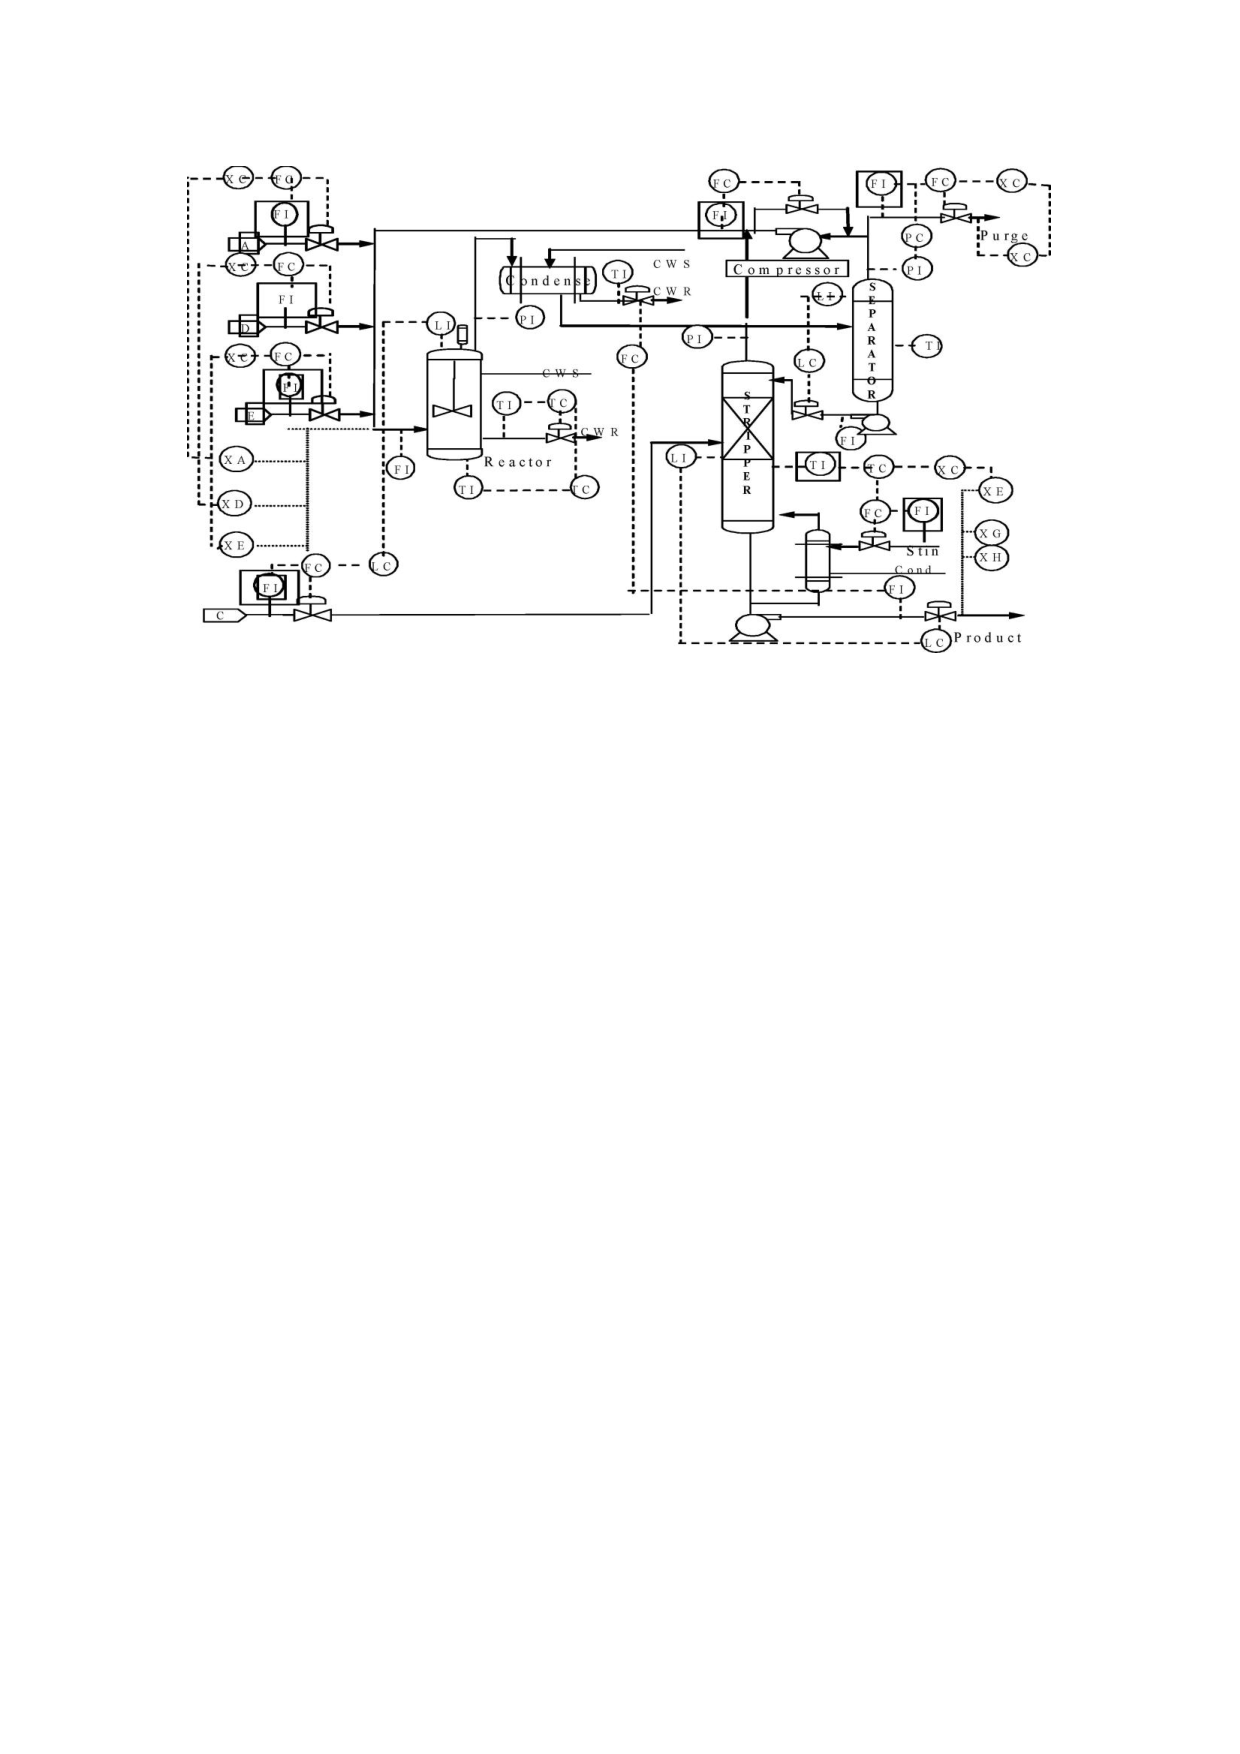
\includegraphics{./Pictures/TE.pdf}
\caption{TE过程的工艺流程图}
\label{TE}
\end{figure}
田纳西伊斯曼(Tennessee Eastman,TE)过程是一个被广泛使用的并且基于真实工业生产过程的仿真平台。许多学者使用该平台来测试其算法的有效性并进行相应的评估,该仿真平台的闭环结构如图\ref{TE} 所示。它包含五个主要的操作部分,分别是:反应器、冷凝器、分离器、解析塔以及压缩机。4种气体反应物(A、C、D、E)经过反应生成2种液体产物(G和H),此外,该过程还包含了1种副产物(F)及惰性气体(B) ,其中,B未直接参与反应。整个过程的化学方程式如下所示:
\begin{equation}
A(g)+C(g)+D(g)\rightarrow G(liq)
\end{equation}
\begin{equation}
A(g)+C(g)+E(g)\rightarrow H(liq)
\end{equation}
\begin{equation}
A(g)+E(g)\rightarrow F(liq)
\end{equation}
\begin{equation}
3D(g)\rightarrow 2F(liq)
\end{equation}
在整个反应过程中伴随着热量的变化,利用冷凝水实现热量的转移。其具体过程可参考相应文献。TE过程中包含着41个测量变量和12个操作变量以及21个故障,故障的详细信息如下表所示:
\begin{table}[!htb]%\footnotesize
\centering
\caption{TE过程的故障描述}
\label{TEfault}
\begin{tabular}{c l l }

  \hline \hline
  % after \\: \hline or \cline{col1-col2} \cline{col3-col4} ...
   序号 & 故障描述 & 类型 \\
  \hline
  1 & A/C 进料流量比, B 含量保持不变 & 阶跃变化 \\
  2 & B 含量变化, A/C 进料流量比保持不变 & 阶跃变化 \\
  3 & D 进料温度变化 & 阶跃 \\
  4 & 反应器冷却水入口温度变化 & 阶跃变化 \\
  5 & 冷凝气冷却水入口温度变化 & 阶跃变化 \\
  6 & A 进料不足 & 阶跃变化 \\
  7 & C 注入压力不足 & 阶跃变化 \\
  8 & A、B 、C 三种投料比变化 & 随机变化 \\
  9 & D 进料温度变化 & 随机变化 \\
  10 & C 进料温度变化 & 随机变化 \\
  11 & 反应器冷却水入口温度发生变化 & 随机变化 \\
  12 & 冷凝器冷却水入日温度发生变化   & 随机变化 \\
  13 & 流程动力常数偏移 & 缓慢漂移 \\
  14 & 反应器的冷却水阀口工作不正常 & 粘滞型 \\
  15 & 冷凝器的冷却水阀口工作不正常 & 粘滞型 \\
  16 & 未知 & 未知 \\
  17 & 未知 & 未知 \\
  18 & 未知 & 未知 \\
  19 & 未知 & 未知 \\
  20 & 未知 & 未知 \\
  21 & C进料口处阀口卡死 & 停滞位置 \\
  \hline \hline
\end{tabular}
 \vspace*{-.4cm}
\end{table}
本章中选择了22个连续变量和11个操作变量(除了搅拌速率)来模拟反应过程,故障信息见表\ref{process var}所示。其中,训练数据为正常工况下的数据(包含500个样本),所有故障数据在非正常工况下采集(包含960个样本),所有数据的采样间隔均为3 分钟,且故障是在第161 个点也就是在正常工况8小时之后引入故障。
\begin{table*}[!htb]
\caption{TE过程中的监测变量}
\label{process var}
\centering
\begin{tabular}{c l c l c l}
  \hline \hline
  序号   & 变量名称 & 序号   & 变量名称 & 序号   & 变量名称\\
  \hline
  1 & A 流量 &  12 & 气液分离器液位 & 23 & D 进料量  \\
  2 & D 流量 &  13 & 气液分离器压力 & 24 & E 进料量\\
  3 & E 流量 &  14 & 汽提塔分离器出口流量 &25 & A 进料量\\
  4 & 总进料流量 &15 & 汽提塔液位 & 26 & 总进料量\\
  5 & 压缩机返回物料流量 &16 & 汽提塔压力 &27 & 压缩机再循环阀\\
  6 & 反应器给料流量 &17 & 汽提塔出口流量 &28 & 排放阀\\
  7 & 反应器压力 &18 & 汽提塔温度 & 29 & 分离器罐液流量\\
  8 & 反应器液位     &19 & 汽提塔蒸汽流量 & 30 & 汽提塔液体产品流量\\
  9 & 反应器温度 &20 & 压缩机功率 & 31 & 汽提塔水流阀    \\
  10 & 排空物料流量 &21 & 反应器冷凝液出口温度& 32 & 反应器冷水流量\\
  11 & 气液分离器温度 &22 & 冷凝器冷凝液出口温度 & 33 & 冷凝器冷却水流量\\
  \hline \hline
\end{tabular}
 \vspace*{-.3cm}
\end{table*}
本章的TE仿真当中,共选取了11个KECA子模型,也就是$B=11$,此外,选取了两个KECA 的模型用来多对比,其核参数分别是$c=10m$和$c=7000$,在所有的模型当中用来计算$T^2$ 和 SPE 的成分的个数分别为15和20,所有的置信水平为99\%。
\begin{table}[!htb]
\centering
\caption{三种方法的误报率}
\label{Alamrate}
\begin{tabular}{cccc}
\hline\hline
   Statistics & KECA($c=10m$) & KECA($c=10m$) & EKECA   \\
 \hline
 $T^2$ & 0.0638 & 0.0675 & 0.0700 \\
 SPE & 0.0088 & 0.0088 & 0.0250 \\
 \hline\hline
\end{tabular}
\end{table}

\begin{table}[!htb]
\centering
\caption{三种模型的故障检测率}
\label{Derate}
\begin{tabular}{ccccccccc}
\hline\hline
 \multirow{2}{*}{故障类型} &
 \multicolumn{2}{c}{KECA($c=10m$)} &
 \multicolumn{2}{c}{KECA($c=7000$)} &
 \multicolumn{2}{c}{EKECA}\\
 \cline{2-7}
  & $T^2$ & SPE & $T^2$ & SPE & $T^2$ & SPE   \\
 \hline
 1& 0.8125 & 0.0188 & 0.9925 & 0.9925 & 0.9975 & 0.9975 \\
 2& 0.0275 & 0.0038 & 0.9825 & 0.9838 & 0.9850 & 0.9813 \\
 3& 0.1350 & 0.0238 & 0.1600 & 0.0250 & 0.1700 & 0.0663 \\
 4& 0.2813 & \textbf{0.9275}	& 0.3438 & 0.1650 & \textbf{0.9713} &0.9125 \\
 5& 0.3200 & 0.0988 & 0.3638 & 0.2338 &\textbf{1} & \textbf{1}      \\	
 6& 0.0138 & 0      & \textbf{1}      & 0.9975 & \textbf{1}      & \textbf{1}      \\		
 7& 0.4788 & 0.0425 & 0.9575 & \textbf{0.9950} & \textbf{0.9963} & 0.9775      \\		
 8& 0.7888 & 0.3525 & 0.9688 & 0.9638 & 0.9825 & 0.9825 \\		
 9& 0.1075 & 0.0250 & 0.1213 & 0.0138 & 0.1475 & 0.0650 \\	
10& 0.5425 & 0.1113 & 0.7250 & 0.2325 & \textbf{0.8338} & \textbf{0.8875} \\		
11& 0.4250 & 0.4050 & 0.4763 & 0.3413 & \textbf{0.7050} & \textbf{0.6225} \\		
12& 0.7763 & 0.1725 & 0.9875 & 0.9588 & 0.9975 & 0.9988 \\		
13& 0.4175 & 0.2438 & 0.9438 & 0.9238 & 0.9513 & 0.9550 \\
14& 0.7075 & 0.4238 & 0.9300 & 0.9575 & 0.9838 & 0.9988 \\
15& 0.1813 & 0.0313 & 0.1750 & 0.0200 & 0.2075 & 0.0725 \\
16& 0.4150 & 0.1275 & 0.9200 & 0.2850 & 0.9325 & \textbf{0.8363} \\
17& 0.3588 & 0.4913 & 0.8438 & 0.7625 & \textbf{0.9338} & \textbf{0.9575} \\
18& 0.0425 & 0.0300 & 0.8975 & 0.8863 & 0.9100 & 0.9075 \\
19& 0.0863 & 0.0350 & 0.7963 & 0.0438 & 0.7863 & \textbf{0.6588} \\
20& 0.5138 & 0.3225 & 0.7550 & 0.3438 & 0.7263 & 0.7788 \\
21& 0.3500 & 0.5563 & 0.3738 & 0.3588 & 0.4100 & \textbf{0.5413} \\
  \hline\hline
\end{tabular}
\end{table}
\begin{figure}[!htb]
  \centering
   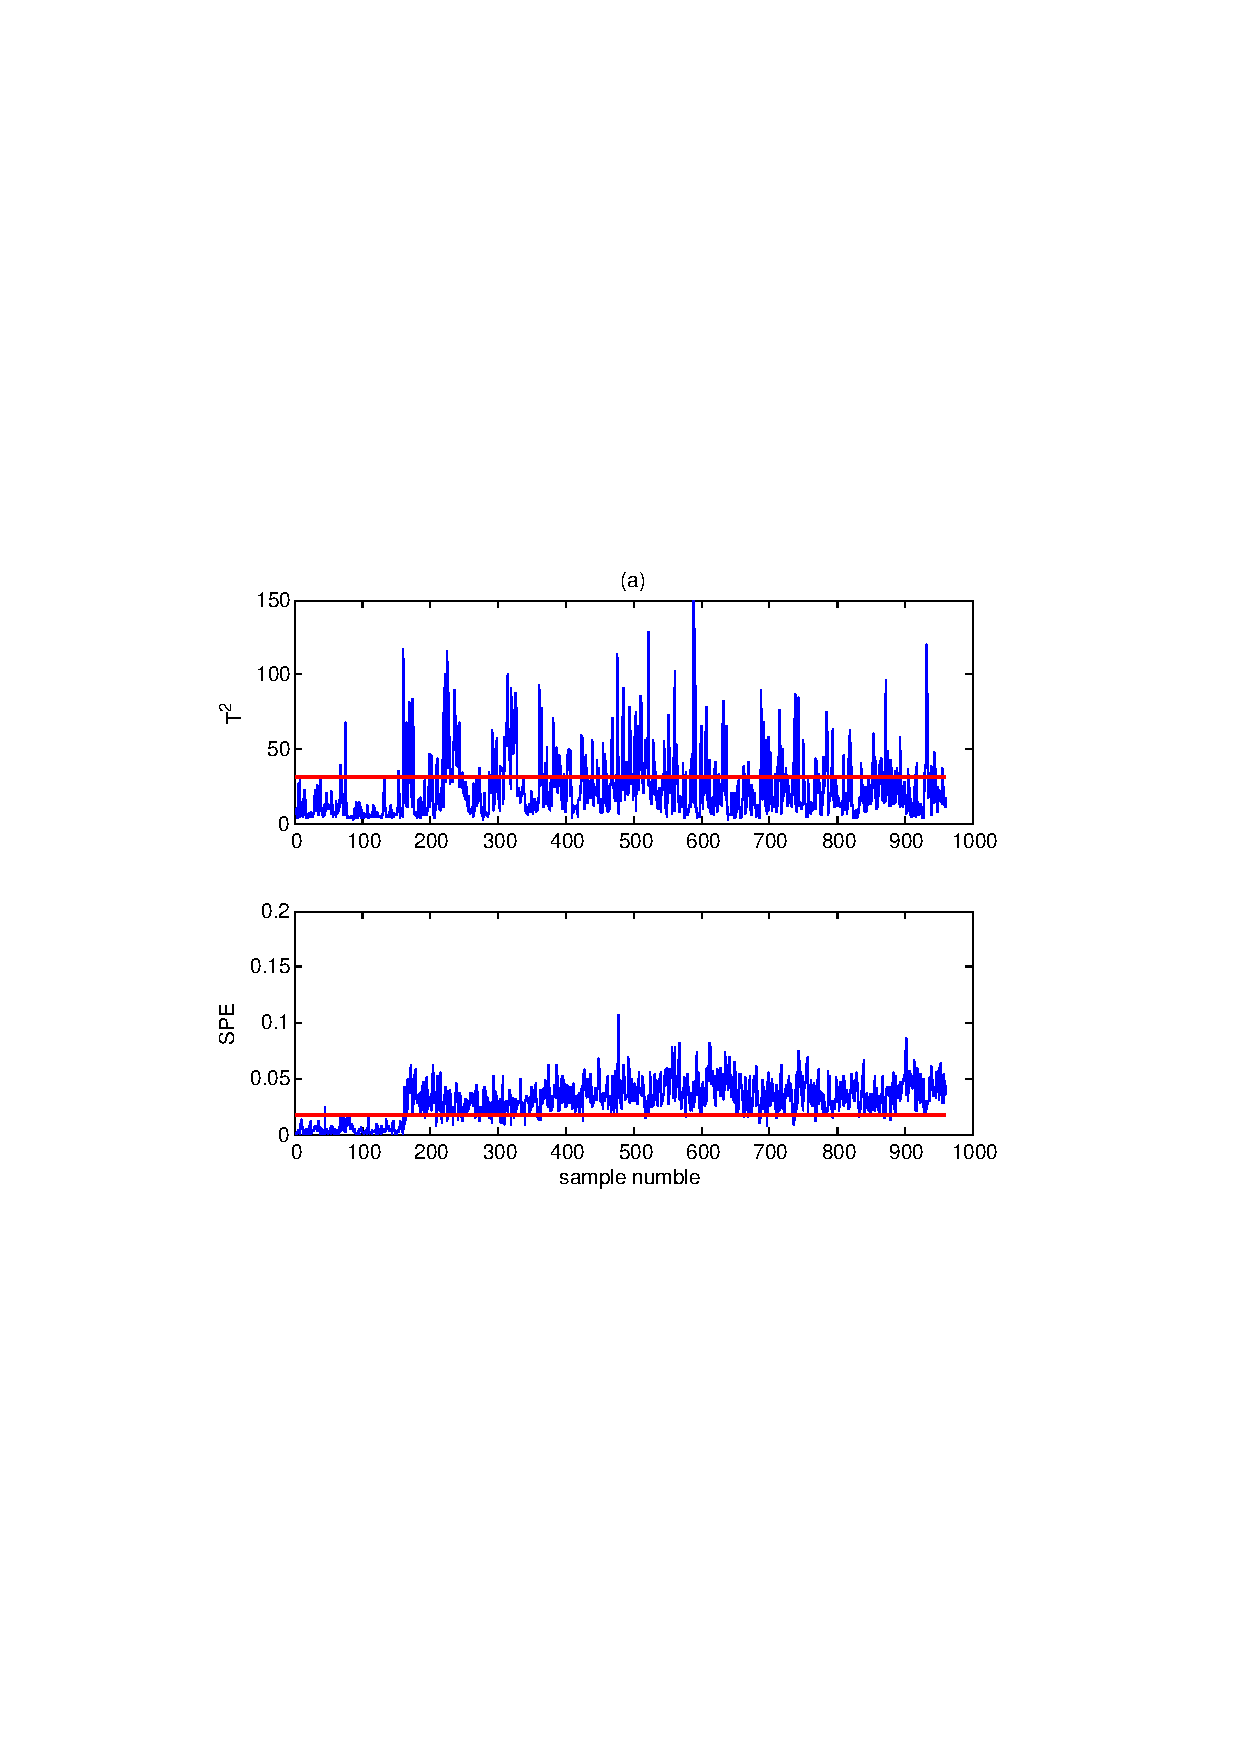
\includegraphics[width=3in]{./Pictures/4-1.pdf}
  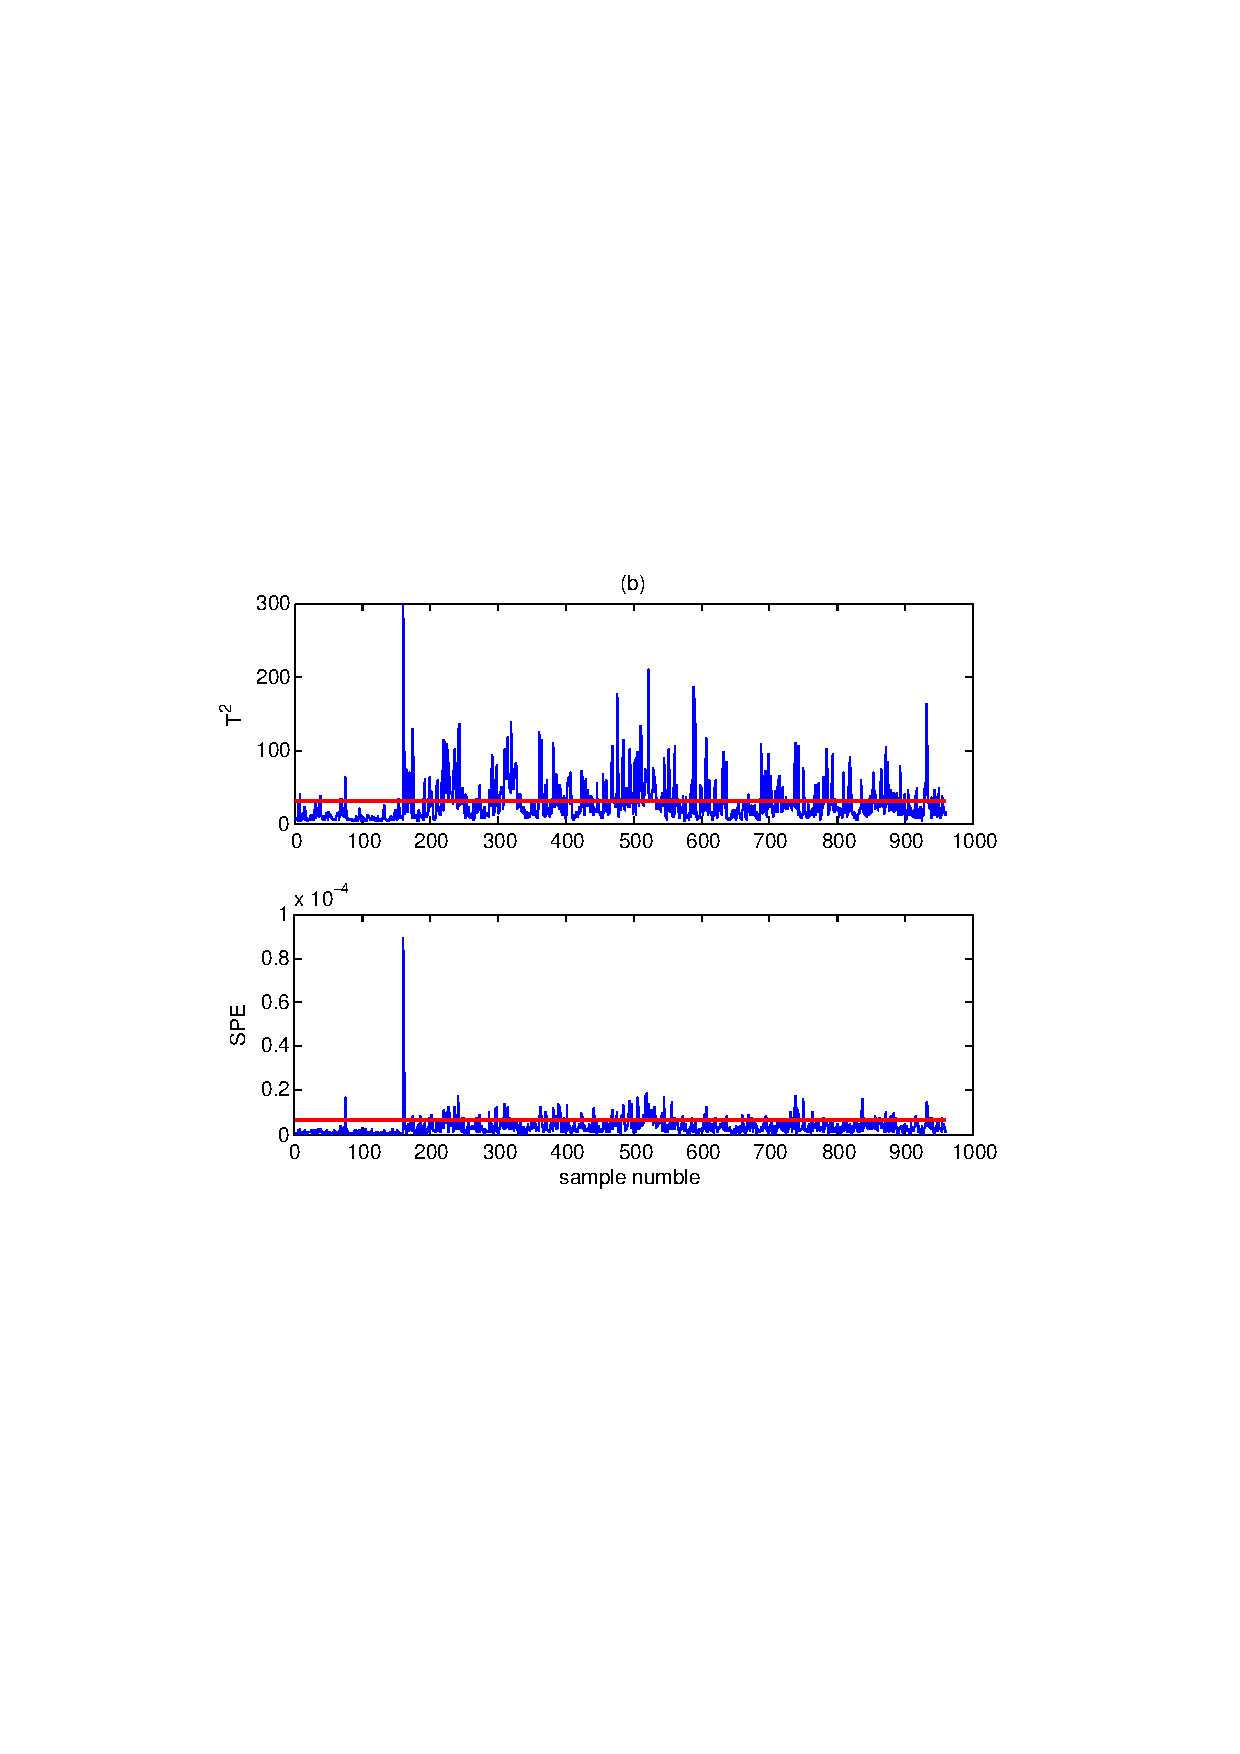
\includegraphics[width=3in]{./Pictures/4-2.pdf}
  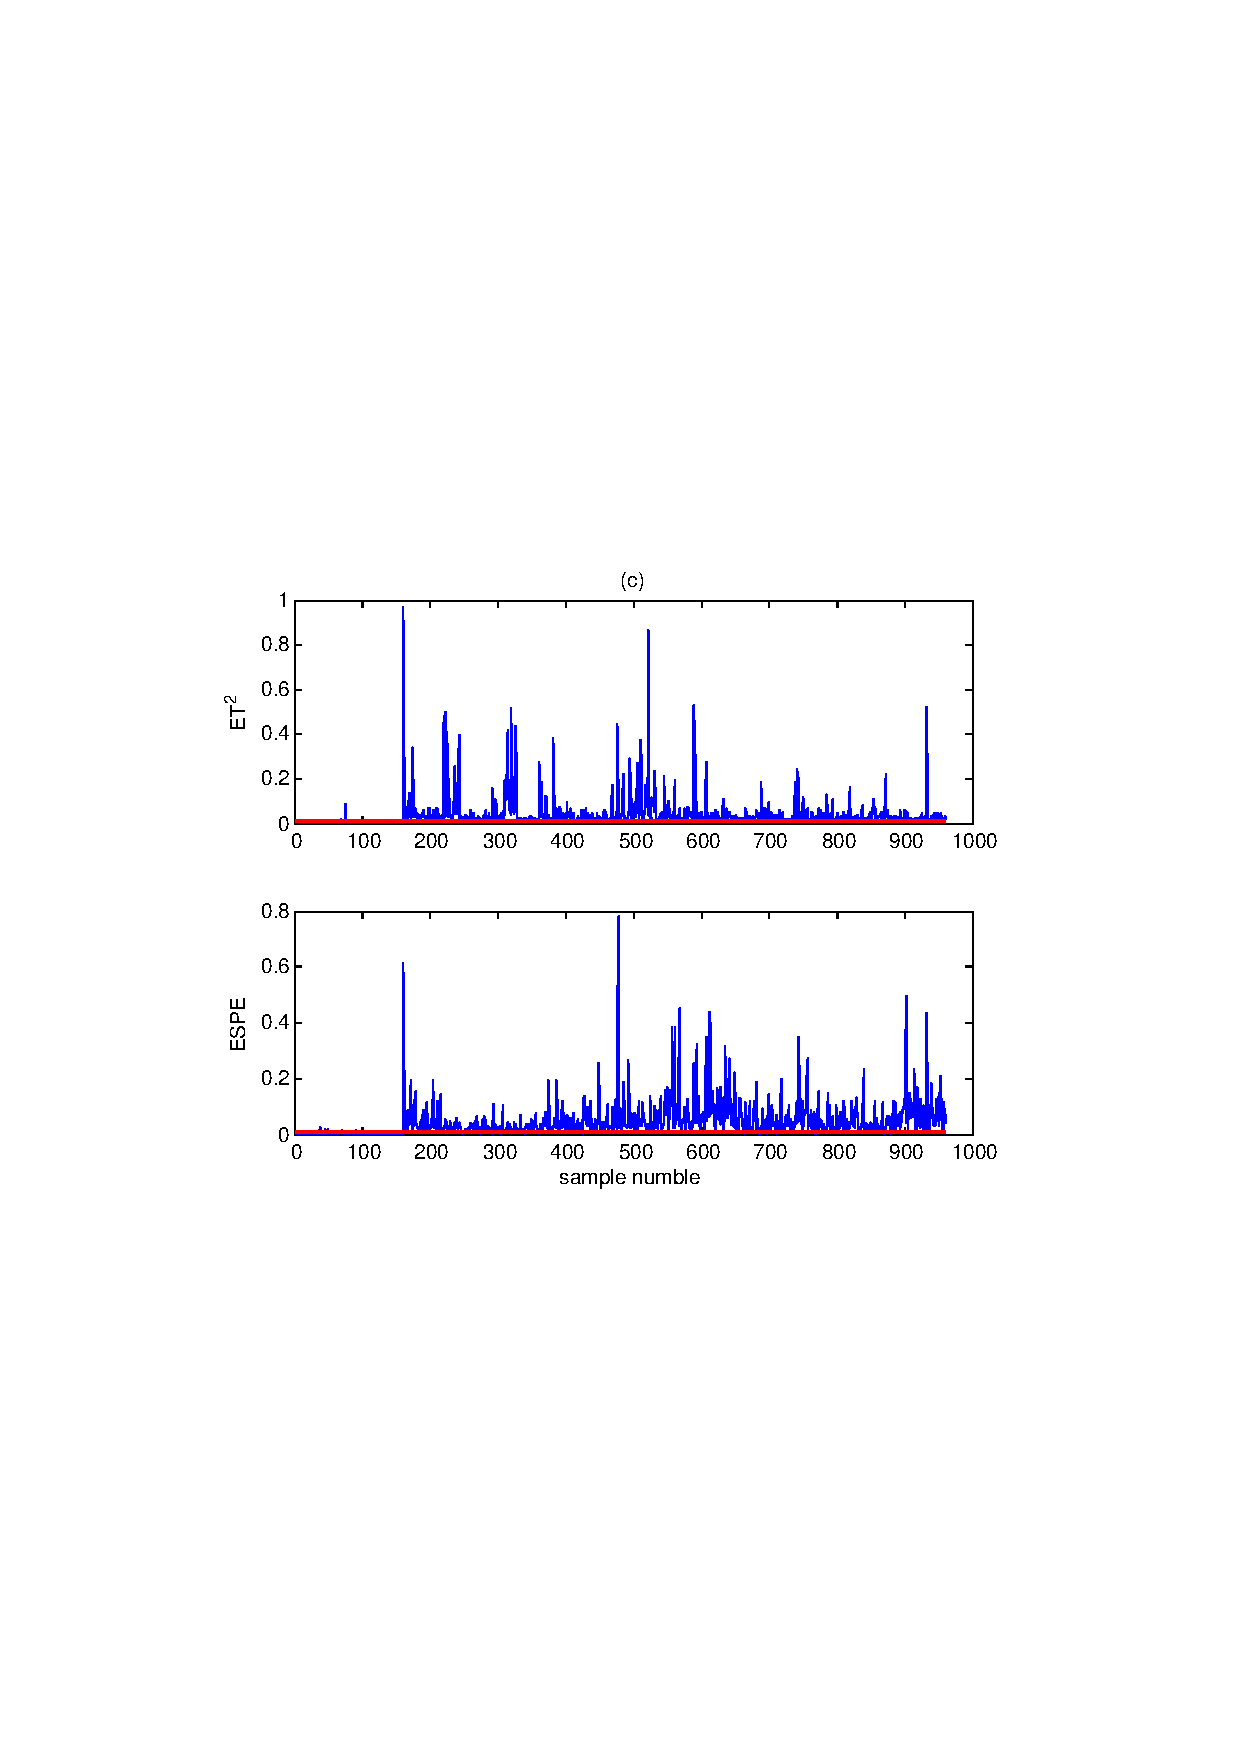
\includegraphics[width=3in]{./Pictures/4-3.pdf}
  \caption{故障4的检测效果: (a) KECA ($c=10m$); (b) KECA (c=7000); (c) EKECA}\label{fault4}
  \vspace*{-0.4cm}
\end{figure}
\begin{figure}[!htb]
  \centering
   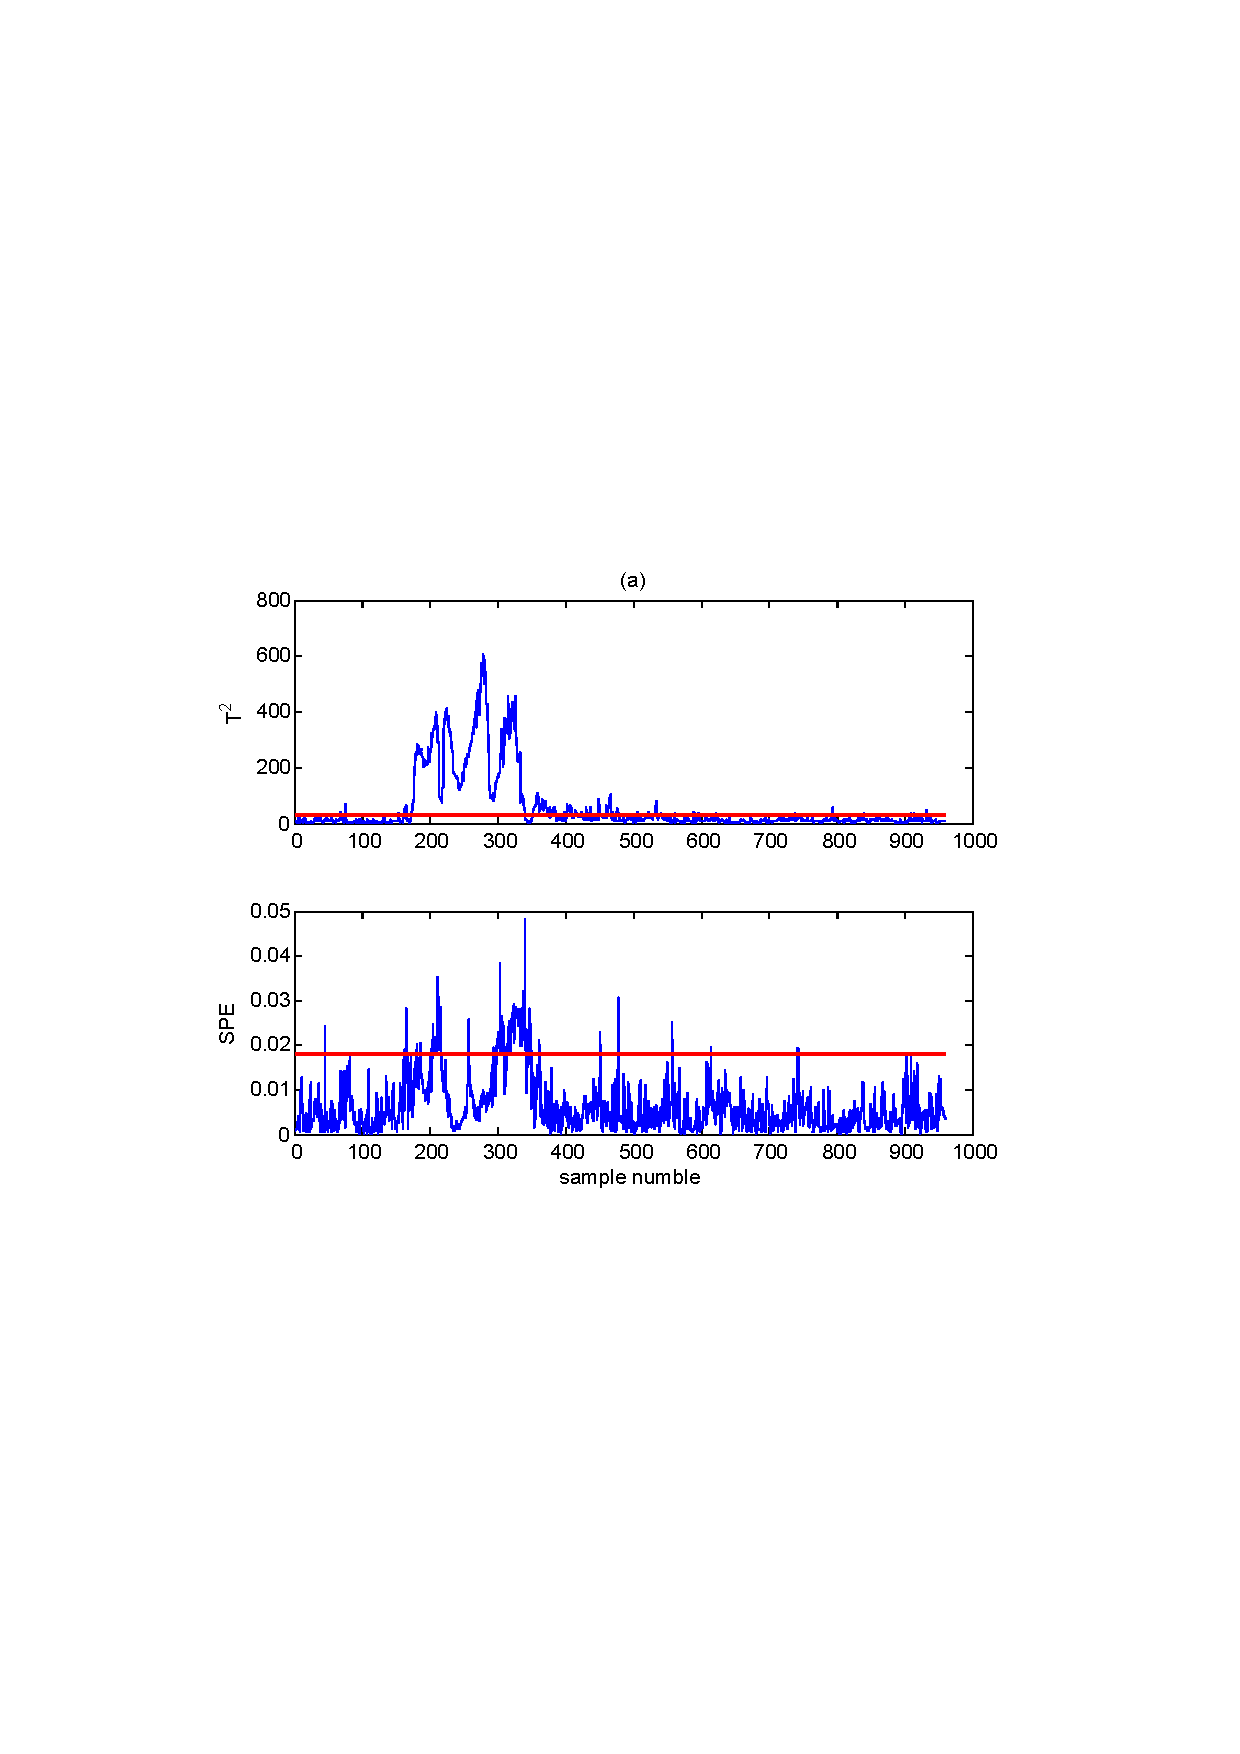
\includegraphics[width=3in]{./Pictures/5-1.pdf}
  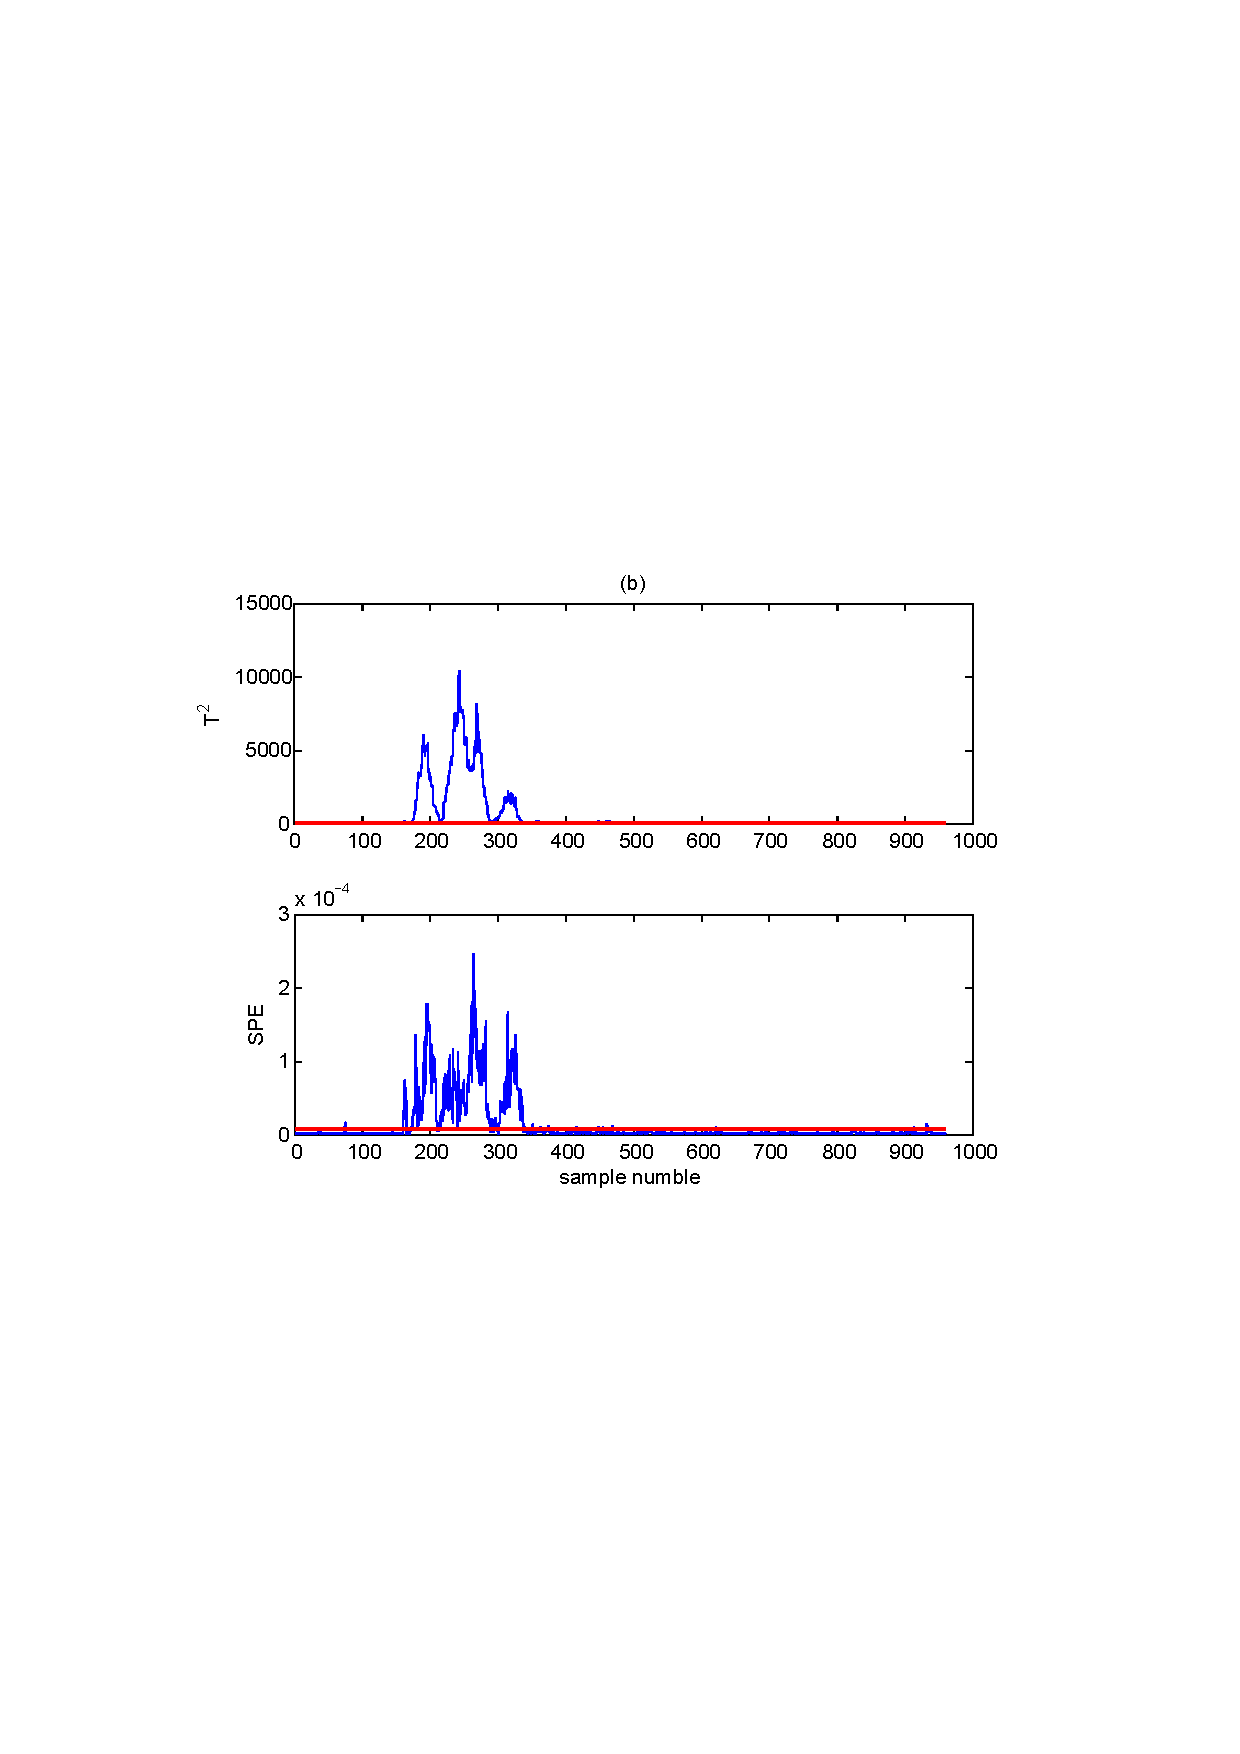
\includegraphics[width=3in]{./Pictures/5-2.pdf}
  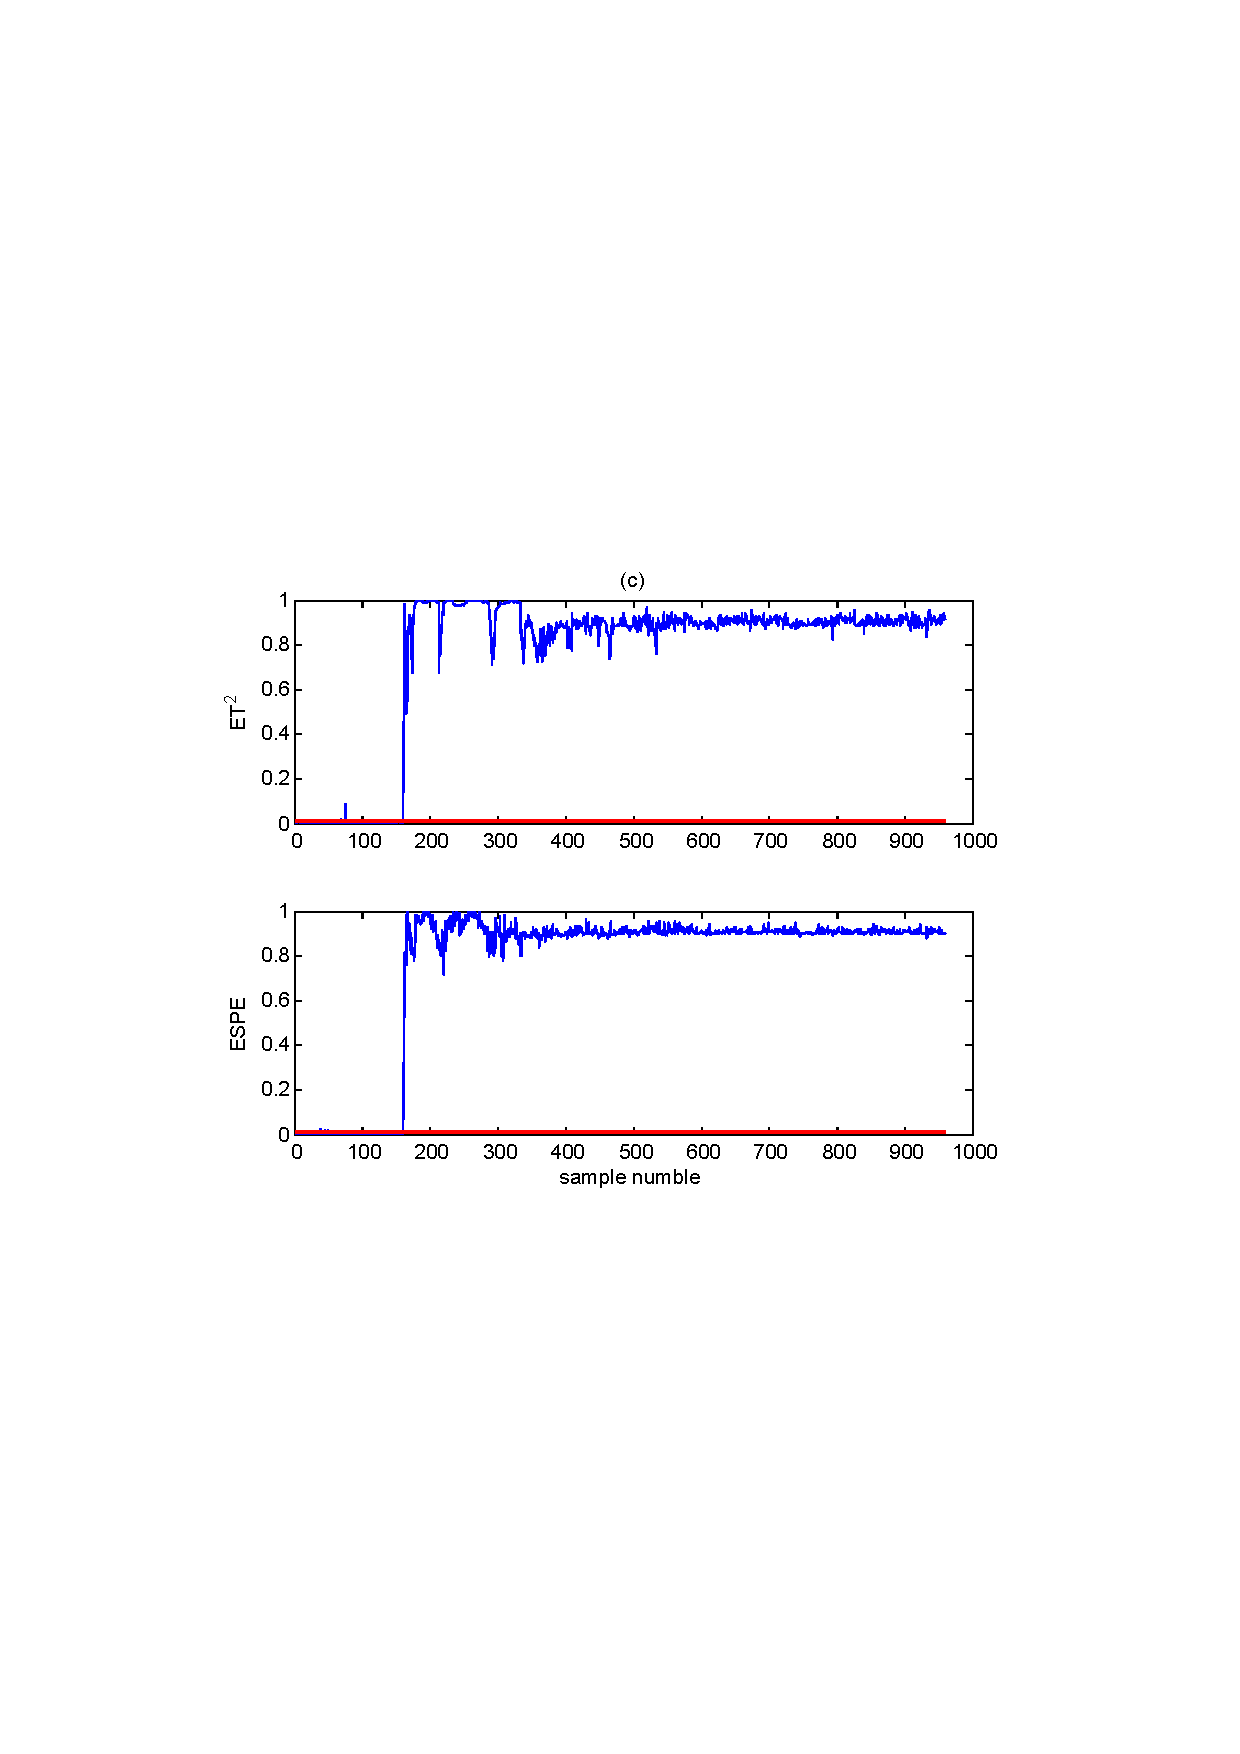
\includegraphics[width=3in]{./Pictures/5-3.pdf}
  \caption{故障5的检测效果: (a) KECA ($c=10m$); (b) KECA (c=7000); (c) EKECA}\label{fault5}
  \vspace*{-0.4cm}
\end{figure}

为了说明EKECA方法的可行性,对正常工况下的数据进行监测,其监测效果如表\ref{Alamrate} 所示,这三种方法的误报率均比较低,从而验证了这三种方法的有效性。21种故障的检测率如表\ref{Derate}所示,其中检测效果最好的部分用黑体标了出来。从表中的仿真结构不难看出,EKECA与单独参数的KECA相比能够有效地检测大部分故障(故障3,9,15为缓变故障,至今几乎所有算法均没有好的检测效果), 且对某些故障有着非常好的检测效果。以故障4和故障5为例,故障4是阶跃型的故障,由表\ref{TEfault}可知,该故障影响反应器的冷却水的温度变化,从图\ref{fault4}中可以看出,在冷却水的温度变化发生变化时候,EKECA可以有效地检测出该变化,而另外两个模型并不能连续地检测出来,这是因为TE过程是一个闭环系统,当温度发生变化时候,其闭环的作用掩盖了故障的存在,使得单核参数的KECA算法误认为该故障已经消失,其统计指标在控制限上下来回震荡。而EKECA则通过不同类型的参数的集成,能够有效地识别这个存在于闭环中的阶跃故障,在161个采样点之后,两个统计指标均一直处于控制限的上方,实时地显示故障并没有消失。故障5的检测效果如图\ref{fault5}所示,同样从表\ref{TEfault}可知,故障5位冷凝器冷却水入口温度变化所引起的阶跃故障,在第350个采样点之后闭环有效地掩盖了故障存在的事实,使得两个单核参数KECA 都认为故障已经消失,生产过程恢复正常工况,其统计指标均已处于控制限的下方。而EKECA此时依旧能够清晰地指出故障存在的事实,其统计指标均始终处于控制限的上方。EKECA不仅能够针对不同类型的故障均具备较好的检测效果,对于特定类型的故障,EKECA能够有效地持续地检测到故障的存在。
\section{本章小结}
针对工业过程中数据的非线性,本章提出了基于集成学习和贝叶斯推论的KECA检测方法EKECA。 在TE平台上,该方法的仿真结果证实了EKECA相比于单核参数的KECA能够针对不同类型的故障均具备较好的检测效果,对于特定类型的故障也能够有效地持续地检测到故障的存在,可以得到这样的结论:EKECA的故障检测效果优于单模型的KECA。另一方面,该方法也通过集成的手段避免了引入核函数带来的核参数选择难题。同时,使用该方法选择主成分的个数是少于KPCA的,这也使得该方法在处理非线性检测时候速度要优于KPCA。此外,由于该方法的集成性,使得它更能满足未知故障的检测。
